% sos2cayley astar_bomega.sos --rename a=a,!a=b
% Hand-placed on the shared grid (see figures.md): the word classes on a square,
% the root close above it. Styles are centralized in the \tikzset below:
% edit a style to restyle, edit a coordinate to move a node.
\documentclass[tikz,border=4pt]{standalone}
\usetikzlibrary{arrows.meta,shapes.misc}
\begin{document}
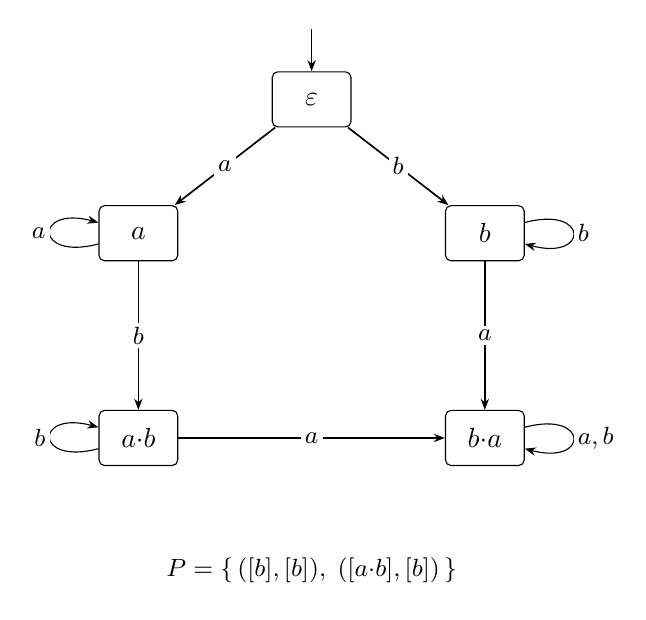
\begin{tikzpicture}[
  class/.style     = {draw, thin, rounded corners=2pt, inner sep=3pt,
                      minimum width=10mm, minimum height=7mm},
  root/.style      = {},          % the root needs no ink: the init stub says it
  init/.style      = {semithick, -{Stealth[length=4pt,width=3pt]}},
  tree/.style      = {semithick, -{Stealth[length=4pt,width=3pt]}},
  nontree/.style   = {thin, -{Stealth[length=4pt,width=3pt]}},
  lbl/.style       = {font=\small, inner sep=1.5pt, fill=white},
  pairs/.style     = {anchor=north, font=\small},
]

  \node[class,root] (eps) at (2.2,2.6) {$\varepsilon$};
  \node[class] (a)   at (0.0,0.9) {$a$};
  \node[class] (b)   at (4.4,0.9) {$b$};
  \node[class]      (ab)  at (0.0,-1.7) {$a{\cdot}b$};
  \node[class] (ba)  at (4.4,-1.7) {$b{\cdot}a$};

  % the root is the adjoined identity: a source, marked like an initial state
  \draw[init] (2.2,3.5) -- (eps);

  \draw[tree]    (eps) to node[lbl] {$a$} (a);
  \draw[tree]    (eps) to node[lbl] {$b$} (b);
  \draw[nontree] (a)  to[loop left]  node[lbl] {$a$} (a);
  \draw[tree]    (a)  to             node[lbl] {$b$} (ab);
  \draw[tree]    (b)  to             node[lbl] {$a$} (ba);
  \draw[nontree] (b)  to[loop right] node[lbl] {$b$} (b);
  \draw[nontree] (ab) to             node[lbl] {$a$} (ba);
  \draw[nontree] (ab) to[loop left]  node[lbl] {$b$} (ab);
  \draw[nontree] (ba) to[loop right] node[lbl] {$a,b$} (ba);

  \node[pairs] at (2.2,-3.1) {$P = \{\, ([b],[b]),\; ([a{\cdot}b],[b]) \,\}$};
\end{tikzpicture}
\end{document}
